\section{32 - A needle in the haystack}

\textbf{Problema:} Encontrar todas las ocurrencias de una cadena $s$ en otra cadena $t$.

\subsection{Resoluci\'on}

La resoluci\'on es directa usando Knuth-Morris-Pratt. El enunciado anticipa que $t$
es potencialmente muy grande. En lugar de reservar memoria para leer la cadena $t$ completa,
se trabaja con un buffer de tama\~no fijo (e independiente de la entrada).

La elecci\'on del tama\~no del buffer s\'olo modifica el tiempo de ejecuci\'on
en una constante. El tama\~no del buffer incluso podr\'ia ser 1. Esto es posible
porque el algoritmo KMP accede a las posiciones de $t$ de manera creciente.

Primero se construye la funci\'on de falla $F$ asociada a la cadena $s$,
de tal manera que:
$$F(i) = \text{longitud del sufijo m\'as largo de $s[0..i)$ que tambi\'en es prefijo de $s[0..i-1)$}$$

\begin{figure}[H]
\centering
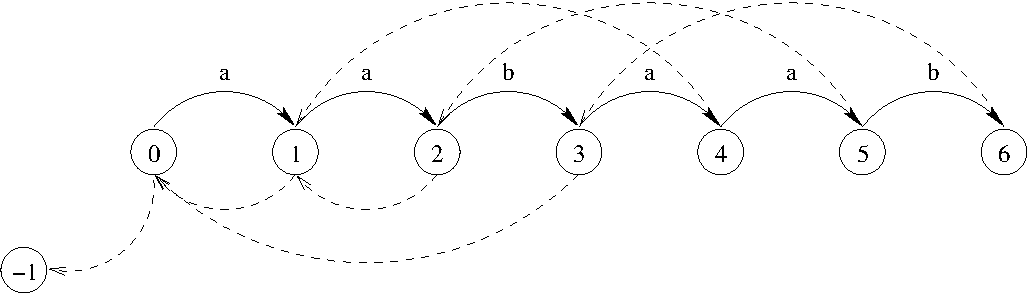
\includegraphics[scale=0.5]{./figuras/kmp.pdf}

\begin{tabular}{l|rrrrrrr}
\hline
$e$    &  0 & 1 & 2 & 3 & 4 & 5 & 6 \\
$F(e)$ & -1 & 0 & 1 & 0 & 1 & 2 & 3 \\
\hline
\end{tabular}
\caption{Aut\'omata impl\'icito en la cadena $aabaab$ (l\'ineas s\'olidas) y la funci\'on de falla $F$ (l\'ineas punteadas)}
\end{figure}

La cadena $s$ y la funci\'on de falla pueden interpretarse como un aut\'omata.
Para buscar las ocurrencias de $s$ en $t$, si se est\'a en el estado $e$ y el
caracter de entrada coincide con $s[e]$, se avanza al estado $e + 1$.
Si el caracter de entrada difiere de $s[e]$, se vuelve al estado $F(e)$
y se repite el proceso. (Si en alg\'un momento se llega al estado -1, el
caracter actual se descarta y se pasa al estado 0).

Dado que la funci\'on de falla cumple que $F(e) < e$ para todo $e$,
y que cada vez que se incrementa el estado se lee un caracter de la
entrada, la cantidad total de retrocesos no puede ser mayor que $|t|$.
Adem\'as, la construcci\'on de la tabla de $F$ es $O(|s|)$. (La
tabla se construye de la manera usual).

Por lo tanto, la complejidad temporal del algoritmo es $O(|s| + |t|)$.
La memoria utilizada es $O(|s|)$ para almacenar la tabla de $F$ y
un buffer de tama\~no constante (64 KB).

\subsection{Implementaci�n}
\noindent
\ttfamily
\shorthandoff{"}\\
\hlstd{}\hlline{\ 1\ }\hldir{\#include\ $<$vector$>$}\\
\hlline{\ 2\ }\hlstd{}\hldir{\#include\ $<$string$>$}\\
\hlline{\ 3\ }\hlstd{}\hldir{\#include\ $<$iostream$>$}\\
\hlline{\ 4\ }\hlstd{}\hldir{\#include\ $<$cassert$>$}\\
\hlline{\ 5\ }\hlstd{}\hldir{\#include\ $<$cstdlib$>$}\\
\hlline{\ 6\ }\hlstd{}\\
\hlline{\ 7\ }\hlkwa{using\ namespace\ }\hlstd{std}\hlsym{;}\\
\hlline{\ 8\ }\hlstd{}\\
\hlline{\ 9\ }\hlkwc{typedef\ }\hlstd{}\hlkwb{unsigned\ long\ long\ int\ }\hlstd{lluint}\hlsym{;}\\
\hlline{10\ }\hlstd{}\hlkwc{typedef\ }\hlstd{vector}\hlsym{$<$}\hlstd{}\hlkwb{int}\hlstd{}\hlsym{$>$\ }\hlstd{vint}\hlsym{;}\\
\hlline{11\ }\hlstd{}\\
\hlline{12\ }\hldir{\#define\ forsn(i,\ s,\ n)\ for\ (int\ i\ =\ (s);\ i\ $<$\ (n);\ i++)}\\
\hlline{13\ }\hlstd{}\hldir{\#define\ forn(i,\ n)\ forsn\ (i,\ 0,\ n)}\\
\hlline{14\ }\hlstd{}\\
\hlline{15\ }\hlslc{//\ Pre\ KMP}\\
\hlline{16\ }\hlstd{}\\
\hlline{17\ }\hlkwb{void\ }\hlstd{}\hlkwd{pkmp}\hlstd{}\hlsym{(}\hlstd{}\hlkwb{const\ }\hlstd{string}\hlsym{\&\ }\hlstd{s}\hlsym{,\ }\hlstd{vint}\hlsym{\&\ }\hlstd{f}\hlsym{)\ \{}\\
\hlline{18\ }\hlstd{\ }\hlkwb{int\ }\hlstd{z\ }\hlsym{=\ }\hlstd{f}\hlsym{{[}}\hlstd{}\hlnum{0}\hlstd{}\hlsym{{]}\ =\ {-}}\hlstd{}\hlnum{1}\hlstd{}\hlsym{;}\\
\hlline{19\ }\hlstd{\ }\hlkwd{forsn\ }\hlstd{}\hlsym{(}\hlstd{i}\hlsym{,\ }\hlstd{}\hlnum{1}\hlstd{}\hlsym{,\ }\hlstd{s}\hlsym{.}\hlstd{}\hlkwd{size}\hlstd{}\hlsym{()\ +\ }\hlstd{}\hlnum{1}\hlstd{}\hlsym{)\ \{}\\
\hlline{20\ }\hlstd{}\hlstd{\ \ }\hlstd{}\hlkwa{while\ }\hlstd{}\hlsym{(}\hlstd{z\ }\hlsym{!=\ {-}}\hlstd{}\hlnum{1\ }\hlstd{}\hlsym{\&\&\ }\hlstd{s}\hlsym{{[}}\hlstd{i\ }\hlsym{{-}\ }\hlstd{}\hlnum{1}\hlstd{}\hlsym{{]}\ !=\ }\hlstd{s}\hlsym{{[}}\hlstd{z}\hlsym{{]})\ }\hlstd{z\ }\hlsym{=\ }\hlstd{f}\hlsym{{[}}\hlstd{z}\hlsym{{]};}\\
\hlline{21\ }\hlstd{}\hlstd{\ \ }\hlstd{f}\hlsym{{[}}\hlstd{i}\hlsym{{]}\ =\ ++}\hlstd{z}\hlsym{;\ }\hlstd{}\hlslc{//\ z\ might\ be\ {-}1}\\
\hlline{22\ }\hlstd{\ }\hlsym{\}}\\
\hlline{23\ }\hlstd{}\hlsym{\}}\\
\hlline{24\ }\hlstd{}\\
\hlline{25\ }\hlslc{//\ Buffer}\\
\hlline{26\ }\hlstd{}\\
\hlline{27\ }\hldir{\#define\ TAMBUF\ 65536}\\
\hlline{28\ }\hlstd{lluint\ pos}\hlsym{;}\\
\hlline{29\ }\hlstd{}\hlkwb{char\ }\hlstd{buf}\hlsym{{[}}\hlstd{TAMBUF}\hlsym{{]};}\\
\hlline{30\ }\hlstd{}\hlkwb{int\ }\hlstd{buf\textunderscore size}\hlsym{;}\\
\hlline{31\ }\hlstd{}\\
\hlline{32\ }\hldir{\#define\ buf\textunderscore sync()\ \{\ $\backslash$}\\
\hlline{33\ }\hldir{\ cin.getline(buf,\ TAMBUF\ +\ 1);\ $\backslash$}\\
\hlline{34\ }\hldir{\ pos\ +=\ buf\textunderscore size;\ $\backslash$}\\
\hlline{35\ }\hldir{\ buf\textunderscore size\ =\ cin.gcount();\ $\backslash$}\\
\hlline{36\ }\hldir{\ cin.clear();\ $\backslash$}\\
\hlline{37\ }\hldir{\}}\\
\hlline{38\ }\hlstd{}\\
\hlline{39\ }\hldir{\#define\ buf\textunderscore start()\ \{\ $\backslash$}\\
\hlline{40\ }\hldir{\ buf\textunderscore sync();\ $\backslash$}\\
\hlline{41\ }\hldir{\ pos\ =\ 0;\ $\backslash$}\\
\hlline{42\ }\hldir{\}}\\
\hlline{43\ }\hlstd{}\\
\hlline{44\ }\hlslc{//\ KMP}\\
\hlline{45\ }\hlstd{}\\
\hlline{46\ }\hlkwb{void\ }\hlstd{}\hlkwd{kmp}\hlstd{}\hlsym{(}\hlstd{}\hlkwb{const\ }\hlstd{string}\hlsym{\&\ }\hlstd{s}\hlsym{,\ }\hlstd{vint}\hlsym{\&\ }\hlstd{f}\hlsym{)\ \{}\\
\hlline{47\ }\hlstd{\ }\hlkwd{buf\textunderscore start}\hlstd{}\hlsym{();}\\
\hlline{48\ }\hlstd{\ }\hlkwb{const\ int\ }\hlstd{final\ }\hlsym{=\ }\hlstd{s}\hlsym{.}\hlstd{}\hlkwd{size}\hlstd{}\hlsym{();}\\
\hlline{49\ }\hlstd{\ }\hlkwb{int\ }\hlstd{state\ }\hlsym{=\ }\hlstd{}\hlnum{0}\hlstd{}\hlsym{;}\\
\hlline{50\ }\hlstd{\ }\hlkwa{while\ }\hlstd{}\hlsym{(}\hlstd{}\hlkwa{true}\hlstd{}\hlsym{)\ \{}\\
\hlline{51\ }\hlstd{}\hlstd{\ \ }\hlstd{}\hlkwd{forn\ }\hlstd{}\hlsym{(}\hlstd{i}\hlsym{,\ }\hlstd{buf\textunderscore size}\hlsym{)\ \{}\\
\hlline{52\ }\hlstd{}\hlstd{\ \ \ }\hlstd{}\hlkwa{if\ }\hlstd{}\hlsym{(}\hlstd{state\ }\hlsym{==\ }\hlstd{final}\hlsym{)\ \{}\\
\hlline{53\ }\hlstd{}\hlstd{\ \ \ \ }\hlstd{cout\ }\hlsym{$<$$<$\ (}\hlstd{pos\ }\hlsym{+\ }\hlstd{i\ }\hlsym{{-}\ }\hlstd{final}\hlsym{)\ $<$$<$\ }\hlstd{}\hlstr{"\ "}\hlstd{}\hlsym{;}\\
\hlline{54\ }\hlstd{}\hlstd{\ \ \ }\hlstd{}\hlsym{\}}\\
\hlline{55\ }\hlstd{}\hlstd{\ \ \ }\hlstd{}\hlkwa{while\ }\hlstd{}\hlsym{(}\hlstd{s}\hlsym{{[}}\hlstd{state}\hlsym{{]}\ !=\ }\hlstd{buf}\hlsym{{[}}\hlstd{i}\hlsym{{]})\ \{}\\
\hlline{56\ }\hlstd{}\hlstd{\ \ \ \ }\hlstd{state\ }\hlsym{=\ }\hlstd{f}\hlsym{{[}}\hlstd{state}\hlsym{{]};}\\
\hlline{57\ }\hlstd{}\hlstd{\ \ \ \ }\hlstd{}\hlkwa{if\ }\hlstd{}\hlsym{(}\hlstd{state\ }\hlsym{==\ {-}}\hlstd{}\hlnum{1}\hlstd{}\hlsym{)\ }\hlstd{}\hlkwa{break}\hlstd{}\hlsym{;}\\
\hlline{58\ }\hlstd{}\hlstd{\ \ \ }\hlstd{}\hlsym{\}}\\
\hlline{59\ }\hlstd{}\hlstd{\ \ \ }\hlstd{state}\hlsym{++;}\\
\hlline{60\ }\hlstd{}\hlstd{\ \ }\hlstd{}\hlsym{\}}\\
\hlline{61\ }\hlstd{}\hlstd{\ \ }\hlstd{}\hlkwa{if\ }\hlstd{}\hlsym{(}\hlstd{buf\textunderscore size\ }\hlsym{$<$\ }\hlstd{TAMBUF}\hlsym{)\ }\hlstd{}\hlkwa{break}\hlstd{}\hlsym{;}\\
\hlline{62\ }\hlstd{}\hlstd{\ \ }\hlstd{}\hlkwd{buf\textunderscore sync}\hlstd{}\hlsym{();}\\
\hlline{63\ }\hlstd{\ }\hlsym{\}}\\
\hlline{64\ }\hlstd{}\hlsym{\}}\\
\hlline{65\ }\hlstd{}\\
\hlline{66\ }\hlkwb{int\ }\hlstd{}\hlkwd{main}\hlstd{}\hlsym{()\ \{}\\
\hlline{67\ }\hlstd{\ }\hlkwa{for\ }\hlstd{}\hlsym{(;;)\ \{}\\
\hlline{68\ }\hlstd{}\hlstd{\ \ }\hlstd{}\hlkwb{int\ }\hlstd{needle\textunderscore size}\hlsym{;}\\
\hlline{69\ }\hlstd{}\hlstd{\ \ }\hlstd{string\ needle}\hlsym{;}\\
\hlline{70\ }\hlstd{}\hlstd{\ \ }\hlstd{cin\ }\hlsym{$>$$>$\ }\hlstd{needle\textunderscore size}\hlsym{;}\\
\hlline{71\ }\hlstd{}\hlstd{\ \ }\hlstd{}\hlkwa{if\ }\hlstd{}\hlsym{(}\hlstd{cin}\hlsym{.}\hlstd{}\hlkwd{eof}\hlstd{}\hlsym{())\ }\hlstd{}\hlkwa{break}\hlstd{}\hlsym{;}\\
\hlline{72\ }\hlstd{}\hlstd{\ \ }\hlstd{cin\ }\hlsym{$>$$>$\ }\hlstd{needle}\hlsym{;}\\
\hlline{73\ }\hlstd{}\hlstd{\ \ }\hlstd{}\hlkwd{assert}\hlstd{}\hlsym{(}\hlstd{needle\textunderscore size\ }\hlsym{==\ }\hlstd{needle}\hlsym{.}\hlstd{}\hlkwd{size}\hlstd{}\hlsym{());}\\
\hlline{74\ }\hlstd{}\hlstd{\ \ }\hlstd{cin}\hlsym{.}\hlstd{}\hlkwd{ignore}\hlstd{}\hlsym{(}\hlstd{}\hlnum{1}\hlstd{}\hlsym{);}\\
\hlline{75\ }\hlstd{\\
\hlline{76\ }}\hlstd{\ \ }\hlstd{vint\ }\hlkwd{f}\hlstd{}\hlsym{(}\hlstd{needle}\hlsym{.}\hlstd{}\hlkwd{size}\hlstd{}\hlsym{()\ +\ }\hlstd{}\hlnum{1}\hlstd{}\hlsym{);}\\
\hlline{77\ }\hlstd{}\hlstd{\ \ }\hlstd{}\hlkwd{pkmp}\hlstd{}\hlsym{(}\hlstd{needle}\hlsym{,\ }\hlstd{f}\hlsym{);}\\
\hlline{78\ }\hlstd{}\hlstd{\ \ }\hlstd{}\hlkwd{kmp}\hlstd{}\hlsym{(}\hlstd{needle}\hlsym{,\ }\hlstd{f}\hlsym{);}\\
\hlline{79\ }\hlstd{}\hlstd{\ \ }\hlstd{cout\ }\hlsym{$<$$<$\ }\hlstd{endl}\hlsym{;}\\
\hlline{80\ }\hlstd{\ }\hlsym{\}}\\
\hlline{81\ }\hlstd{\ }\hlkwa{return\ }\hlstd{}\hlnum{0}\hlstd{}\hlsym{;}\\
\hlline{82\ }\hlstd{}\hlsym{\}}\\
\hlline{83\ }\hlstd{}\\
\mbox{}
\normalfont
\shorthandon{"}

